% Options for packages loaded elsewhere
\PassOptionsToPackage{unicode}{hyperref}
\PassOptionsToPackage{hyphens}{url}
%
\documentclass[
  parskip,
  oneside]{scrreprt}
\usepackage{amsmath,amssymb}
\usepackage{lmodern}
\usepackage{iftex}
\ifPDFTeX
  \usepackage[T1]{fontenc}
  \usepackage[utf8]{inputenc}
  \usepackage{textcomp} % provide euro and other symbols
\else % if luatex or xetex
  \usepackage{unicode-math}
  \defaultfontfeatures{Scale=MatchLowercase}
  \defaultfontfeatures[\rmfamily]{Ligatures=TeX,Scale=1}
\fi
% Use upquote if available, for straight quotes in verbatim environments
\IfFileExists{upquote.sty}{\usepackage{upquote}}{}
\IfFileExists{microtype.sty}{% use microtype if available
  \usepackage[]{microtype}
  \UseMicrotypeSet[protrusion]{basicmath} % disable protrusion for tt fonts
}{}
\makeatletter
\@ifundefined{KOMAClassName}{% if non-KOMA class
  \IfFileExists{parskip.sty}{%
    \usepackage{parskip}
  }{% else
    \setlength{\parindent}{0pt}
    \setlength{\parskip}{6pt plus 2pt minus 1pt}}
}{% if KOMA class
  \KOMAoptions{parskip=half}}
\makeatother
\usepackage{xcolor}
\IfFileExists{xurl.sty}{\usepackage{xurl}}{} % add URL line breaks if available
\IfFileExists{bookmark.sty}{\usepackage{bookmark}}{\usepackage{hyperref}}
\hypersetup{
  pdftitle={Report\_Group4\_Team4},
  pdfauthor={Team 4},
  hidelinks,
  pdfcreator={LaTeX via pandoc}}
\urlstyle{same} % disable monospaced font for URLs
\usepackage{graphicx}
\makeatletter
\def\maxwidth{\ifdim\Gin@nat@width>\linewidth\linewidth\else\Gin@nat@width\fi}
\def\maxheight{\ifdim\Gin@nat@height>\textheight\textheight\else\Gin@nat@height\fi}
\makeatother
% Scale images if necessary, so that they will not overflow the page
% margins by default, and it is still possible to overwrite the defaults
% using explicit options in \includegraphics[width, height, ...]{}
\setkeys{Gin}{width=\maxwidth,height=\maxheight,keepaspectratio}
% Set default figure placement to htbp
\makeatletter
\def\fps@figure{htbp}
\makeatother
\setlength{\emergencystretch}{3em} % prevent overfull lines
\providecommand{\tightlist}{%
  \setlength{\itemsep}{0pt}\setlength{\parskip}{0pt}}
\setcounter{secnumdepth}{5}
\newlength{\cslhangindent}
\setlength{\cslhangindent}{1.5em}
\newlength{\csllabelwidth}
\setlength{\csllabelwidth}{3em}
\newlength{\cslentryspacingunit} % times entry-spacing
\setlength{\cslentryspacingunit}{\parskip}
\newenvironment{CSLReferences}[2] % #1 hanging-ident, #2 entry spacing
 {% don't indent paragraphs
  \setlength{\parindent}{0pt}
  % turn on hanging indent if param 1 is 1
  \ifodd #1
  \let\oldpar\par
  \def\par{\hangindent=\cslhangindent\oldpar}
  \fi
  % set entry spacing
  \setlength{\parskip}{#2\cslentryspacingunit}
 }%
 {}
\usepackage{calc}
\newcommand{\CSLBlock}[1]{#1\hfill\break}
\newcommand{\CSLLeftMargin}[1]{\parbox[t]{\csllabelwidth}{#1}}
\newcommand{\CSLRightInline}[1]{\parbox[t]{\linewidth - \csllabelwidth}{#1}\break}
\newcommand{\CSLIndent}[1]{\hspace{\cslhangindent}#1}
\usepackage[english]{babel}
\usepackage[utf8]{inputenc}
\usepackage[T1]{fontenc}
\usepackage{lmodern}
\usepackage[onehalfspacing]{setspace}
\usepackage[headsepline]{scrlayer-scrpage}
\usepackage{url}
\usepackage[backend=biber, style=authoryear, giveninits=true, maxbibnames=99, uniquename=init, maxcitenames=2, hyperref=true, date=year]{biblatex}
\usepackage{xpatch}
\usepackage{csquotes}
\usepackage{amsmath}
\usepackage{listings}
\usepackage{booktabs}
\usepackage{longtable}
\usepackage{multirow}
\usepackage{rotating}
\usepackage{subfigure}
\usepackage{graphicx}
\usepackage{float}
\usepackage{acronym}
\usepackage{lipsum}
\usepackage{scrhack}
\emergencystretch=50pt
\clubpenalty = 10000
\widowpenalty = 10000
\displaywidowpenalty = 10000
\automark[section]{chapter}
\renewcommand*{\chaptermarkformat}{}
\renewcommand*{\sectionmarkformat}{}
\setkomafont{title}{\sffamily}
\setkomafont{disposition}{\usekomafont{title}}
\setkomafont{author}{\usekomafont{title}}
\setkomafont{date}{\usekomafont{title}}
\setkomafont{caption}{\sffamily\small}
\setkomafont{captionlabel}{\usekomafont{caption}\bfseries\small}
\setkomafont{pagehemad}{\normalfont\scshape}
\ifLuaTeX
  \usepackage{selnolig}  % disable illegal ligatures
\fi

\title{Report\_Group4\_Team4}
\author{Team 4}
\date{7/16/2022}

\begin{document}
\maketitle

\hypertarget{introduction}{%
\chapter{Introduction}\label{introduction}}

Mouse development and organogenesis occurs as early as compaction and
the formation of a blastocyst before preimplantation of the mouse
embryo. After the fertilization the most important stages of development
are the two cell; four cell; eight cell stadium just as the morula and
the blastocyst which already contains three different cell types:
trophectoderm; epiblast and the endoderm (Kojima \emph{et al.}, 2014).
The blastula is roughly reached after 72 hours (Ciemerych and Sicinski,
2005). The very first two cycles after fertilization have a lengthened
duration compared to the fourth and eighth cell stage. This is due to
the chromatin remodeling and the decondensation of maternal and parental
chromatin in order to gain a functional nucleus (Ciemerych and Sicinski,
2005). The dynamic cell changes are controlled by so called D-cyclins,
many transcription factors, and mainly performed by DNA- and Histone
methylases and demethylases (Mihajlović and Bruce, 2017), (Sha \emph{et
al.}, 2019). In the one cell stage and right after the end of the
two-cell stage entering the fourth cell stage, the minor and the major
Zygote Genome Activation (ZGA) onsets (Mihajlović and Bruce, 2017). This
implies that from now on the development will be directed by the
zygote's genome transcripts, while the maternal mRNA transcripts will be
degraded, and thus the expression pattern will drastically change (AOKI,
2022). We will concentrate on the dynamic change of the gene expression
especially in the fourth cell stage. In comparison ZGA takes place
between the fourth and the eight-cell stage in humans (Xie \emph{et
al.}, 2010). Since mammalian embryos develop under low oxygen
conditions, managing these conditions and providing enough oxygen for
morphogenesis and cell proliferation and tissue formation is essential.
In order to prevent hypoxia, a low oxygen condition, while
embryogenesis, there are hypoxia sensitive genes which will be activated
(Dunwoodie, 2009). One of the most important factors for this matter is
the Hypoxia Inducing Factor (HIF). HIF binds to the HIF-Responsive
element, which is encoded by three genes. Whenever HIF is absent or
epigenetically silenced, the morphogenesis of the heart is impaired.
Especially affected is the formation of the endothelium in the
cardiovascular muscles and the chamber formation of the heart. To
conclude, in order to develop a healthy cardiovascular system HIF is
essential (Krishnan \emph{et al.}, 2008). A rather hidden and enigmatic
role plays tissue restricted antigens (TRAs) in embryonic development.
With the aim of establishing functioning T cells, which recognize
intruders as pathogens via T cell receptors (TCRs), the T cells need to
be trained (Alberts \emph{et al.}, 2015). The positive and negative
selection in the thymus allows T cells to recognize self-antigens which
are displayed by MHC molecules on the cell surface. The expression and
regulation are controlled by AIRE autoimmune regulator and Fezf2
(Monteleone-Cassiano \emph{et al.}, 2022). The role of TRAs in the
crucial stages of embryonic development is yet unknown, just as the
immune suppressive impact of Fezf2 regulator in those cells (Takaba and
Takayanagi, 2017).

\hypertarget{materials}{%
\chapter{Materials}\label{materials}}

\hypertarget{r-and-rstudio}{%
\section{1. R and RStudio}\label{r-and-rstudio}}

This project was entirely done in R(R Core Team, 2022) version 4.2.0
(2022-04-22) and RStudio (RStudio Team, 2021) version 2021.09.0. \#\# 2.
Affy Packages The microarray chips used in the the research of Xie
\textbf{et al.} are Affymatrix GeneChips. In order to process and
analyse these chips we used the affy package (Gautier \emph{et al.},
2004) that was installed using Bioconductor. Affy is an R package that
is used to analyse gene chips of the affymatrix type. Some of its many
functions are to read in data and do quality control checks. The data
are read in as .CEL files.

\hypertarget{brainarray-and-loading-the-chip-describtion-files-of-mouse-and-bovine}{%
\section{3. Brainarray and loading the Chip Describtion Files of mouse
and
bovine}\label{brainarray-and-loading-the-chip-describtion-files-of-mouse-and-bovine}}

The chip descritption files (CDF) of our 2 data sets (mouse and bovine)
were downloaded using BrainArray (Dai \emph{et al.}, 2005). Brainarray
is an online data bank that gathers re-analyzed existing Affymatrix
Genechip data ``with updated probe set definitions'', (Dai \emph{et.
al}, 2005) to offer custom cdf files with better gene annotations and
calculations.

\hypertarget{bioconductor}{%
\section{4. Bioconductor}\label{bioconductor}}

Bioconductor (Morgan, 2022) gathers different packages that are used in
R, in order to widen the analysis of gene expression data sets. Most of
the packages that we used in our project are installed through
Bioconductor, this includes: limma, affy,vsn, GSEA and AnnotationDbi.

\hypertarget{tidyverse}{%
\section{5. Tidyverse}\label{tidyverse}}

Tidyverse is a collection of packages used for ``data import, tidying,
manipulation, visualisation, and programming'' (Wickham \emph{et al.},
2019). It is analog to Bioconductor.

\hypertarget{methods}{%
\chapter{Methods}\label{methods}}

\hypertarget{quality-control}{%
\section{1.Quality Control}\label{quality-control}}

\hypertarget{mouse-chips}{%
\subsection{Mouse chips}\label{mouse-chips}}

After reading in the data, we examined the chips of the mouse data set
to see if any of the chips have quality issues. This was done using
different objectives. Firstly, we read the chips as images in order to
see if they differ from the overall expression trend. We noticed three
chips that seemed to differ. The first chip,second cell stage third
replicate, is distinctly over-expressed and the other two, morula second
and third replicate,were under-expressed.

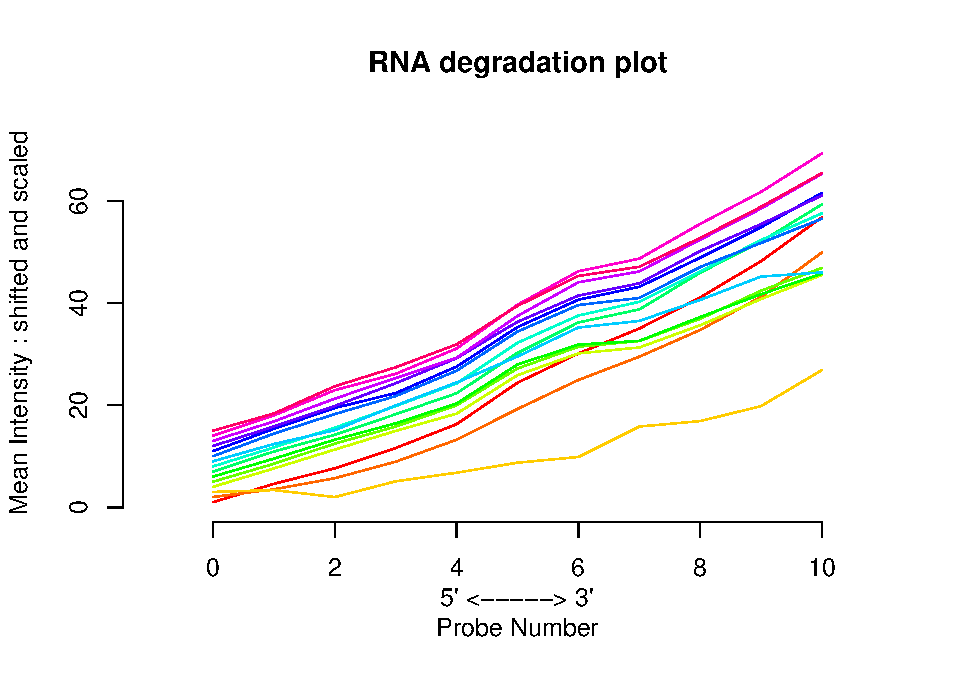
\includegraphics{Layout_Report_Group4_Team4---Kopie_files/figure-latex/unnamed-chunk-5-1.pdf}
The second step in the quality control was done through an RNA
degradationm plot on the data set, that is shifted and scaled. The RNA
degradation plot follows the degradation of the RNA by targeting the
probe set in different regions of the selected transcript, the central
section, the 3 prime and the 5 prime. This allows assessing the
degradation rate of individual transcripts by examining the 3'/5'
probe-set signal ratios. A good RNA degradation plot would show a steady
upward trend with minimal crossing. In our case we can see that the
orange line follows a different trend than the others and that there is
crossing.On the other hand, if we only shift the RNA degradation plot
without scaling, we can't see an effect. This could be due to the three
chips that have low quality.

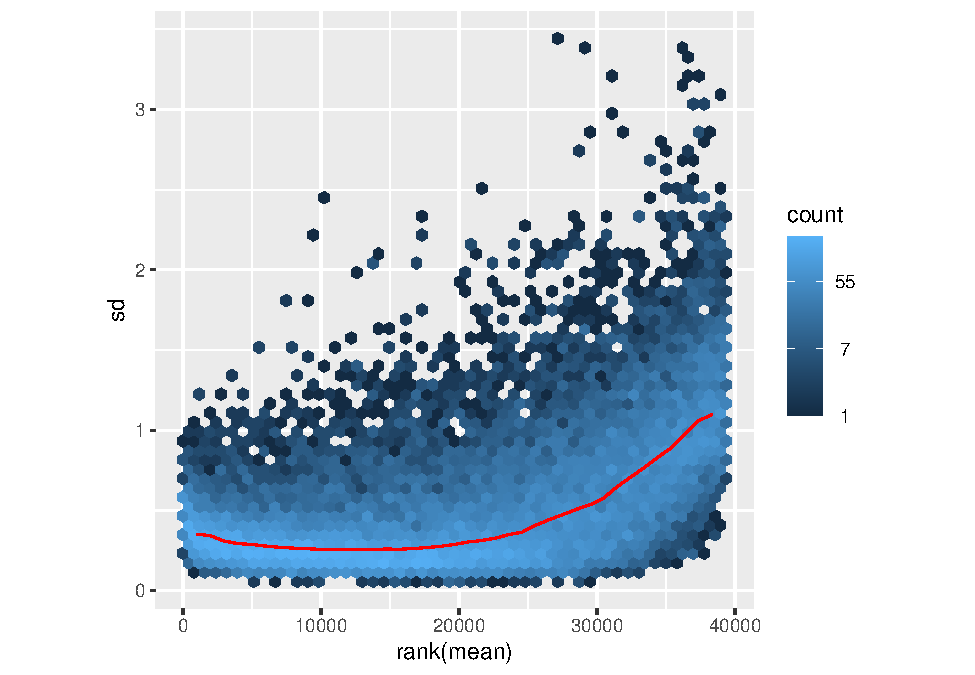
\includegraphics[height=0.25\textheight]{Layout_Report_Group4_Team4---Kopie_files/figure-latex/unnamed-chunk-6-1}

\hypertarget{bovine}{%
\subsection{Bovine}\label{bovine}}

The same procedure was done for the bovine data set. Through the quality
control of the bovine chips, we saw that the last chip had quality
issues, as the dye showed a difference from the rest. This can also be
seen by plotting the RNA degradation plot of the 16 chips, as the 16th
chip (GSM456642) (blastocyst, second replicate) crosses the rest of the
chips.

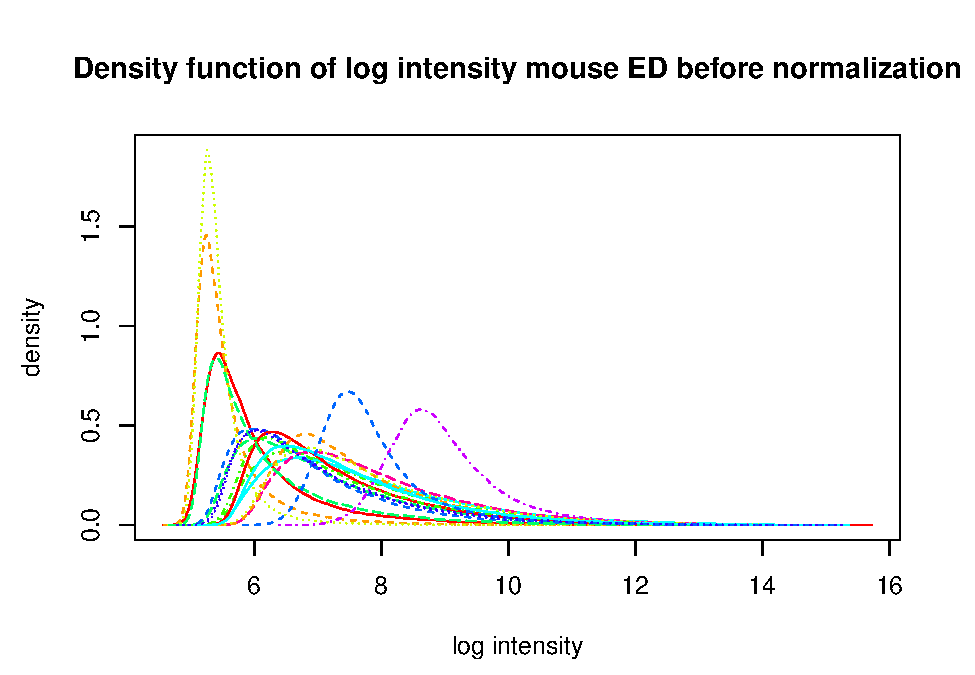
\includegraphics[height=0.2\textheight]{Layout_Report_Group4_Team4---Kopie_files/figure-latex/unnamed-chunk-8-1}

\includegraphics[height=0.25\textheight]{Layout_Report_Group4_Team4---Kopie_files/figure-latex/unnamed-chunk-9-1}

\hypertarget{variance-stabilization-normalization}{%
\section{2.Variance Stabilization
Normalization}\label{variance-stabilization-normalization}}

Variance Stabilization Normalization (vsn) is a stastistical
method,developed by Huber \emph{et al.} (Huber \emph{et al.}, 2002) that
is used for micro-arrays to reduce background noise, optical illusions
and dye irregularities. It is done through a log transformation in order
to get a better concept of perception. It includes three main steps, the
normalization, which is done through data calibration, the mean-
variance- dependance of the the model, and a variance stabilizing
transformation. (Huber \emph{et. al}) For both data sets (mouse and
bovine), the vsn was made visualized using different ploting techniques.

\hypertarget{mean-versus-standard-deviation-plot}{%
\subsection{1. Mean versus Standard deviation
plot}\label{mean-versus-standard-deviation-plot}}

The quality of the vsn can be visualized using the mean versus standard
deviation plot (meanSDplot). The standard deviation should not have a
strong correlation to the mean/variance and thus the red line of the
median estimator should be horizontal. (Dinkelacker 2019)

\hypertarget{density-plot}{%
\subsection{2. Density Plot}\label{density-plot}}

The density plot is used, to plot the density function against the log
intensity of each chip. This way we can confirm if the vsn was succesful
or not. If the curves are well adjusted after the vsn, this would mean
that the normalization was successful. As the QC showed, chips 6,14,15
are of low quality.That's why we will be disregarding them for the rest
of our analysis.

\hypertarget{hierarchical-clustering}{%
\section{3. Hierarchical Clustering}\label{hierarchical-clustering}}

After performing the QC, we proceeded to cluster the 15 chips. We
created a distance matrix using the euclidean distance. After that the
hierarchical clustering was done using the average linkage method. This
was plotted and a dendogram was formed. The bigger the hight difference
the more different the groups are.

\hypertarget{finding-tras-in-our-data-set}{%
\section{4. Finding TRAs in our data
set}\label{finding-tras-in-our-data-set}}

Through the available data set provided by Dinkelacker, we were able to
match the TRAs with our mouse data set using R

\hypertarget{differential-gene-expression-analysis}{%
\section{5. Differential Gene Expression
Analysis}\label{differential-gene-expression-analysis}}

The differential gene expression (dge) analysis ``refers to the analysis
and interpretation of differences in abundance of gene transcripts
within a transcriptome''. (Conesa \emph{et al.}, 2016) (Conesa
\textbf{et al.}, 2016) It is done in R using the limma package provided
by Bioconductor. (Phipson \emph{et al.}, 2016) Limma uses the linear
model as an approach for the dge, by simply forming a design matrix
``which indicates in effect which RNA samples have been applied to each.
array'' (Phipson \textbf{et al.}, 2016) and a contrast matrix, where we
define which objectives will be compared to each other. In our case the
contrast matrix compares cell stages to each other and the design
matrix, desgins a matrix that groups the chips by the cell stage they
belong to. After that a linear model will fitted to our design matrix,
and in the end the contrast matrix will be fit with the linear model.
Limma uses the Bayes method in order to use probability to represent all
uncertainty within the model. Here it moderates the standard errors of
the estimated log-fold changes. It is calculated using the Bayesian
Theorem, which is then used for hypothesis testing, in our case a
t-test. The differential gene expression was performed for the mouse and
bovine data sets respectively.

\hypertarget{gene-set-enrichment-analysis}{%
\section{6. Gene Set Enrichment
Analysis}\label{gene-set-enrichment-analysis}}

A gene set enrichment analysis (GSEA) is used to identify if a set of
genes is enriched in expression. The analysis uses previous knowledge in
order to see if a set of genes is related by shared criteria. This
criteria can be a certain pathway or a functional classification.
(Thomas \emph{et al.}, 2011) The GSEA is based on the results from the
DGE that includes the results of the t-test and the p-values.
Additionally we use The Molecular Signatures Database (MSigDB), which is
a resource that contains annotated gene sets for our species and pathway
analysis. (Dolgalev, 2022) Using the annotation packages for Mus
musculus and Bos taurus gives us information from different identifiers
(Carlson, 2022) For us the GSEA will help us with enriching pathways
that might play a role in tissue formation.

\hypertarget{results}{%
\chapter{Results}\label{results}}

\hypertarget{vsn}{%
\section{1. VSN}\label{vsn}}

\hypertarget{mouse}{%
\subsection{Mouse}\label{mouse}}

After the QC, we proceeded to normalize our data using the variance
stabilization method. To see if the VSN was successful we used two
plotting techniques, the mean versus standard deviation plot and the
density probability against the log intensity. The mean versus standard
deviation, shows a slight upward trend of the red line which represents
the median estimator. If all chips were of good quality, the median
estimator would show a horizontal line.

\includegraphics[height=0.25\textheight]{Layout_Report_Group4_Team4---Kopie_files/figure-latex/unnamed-chunk-10-1}
The density plot shows that all chips align with slight differences.

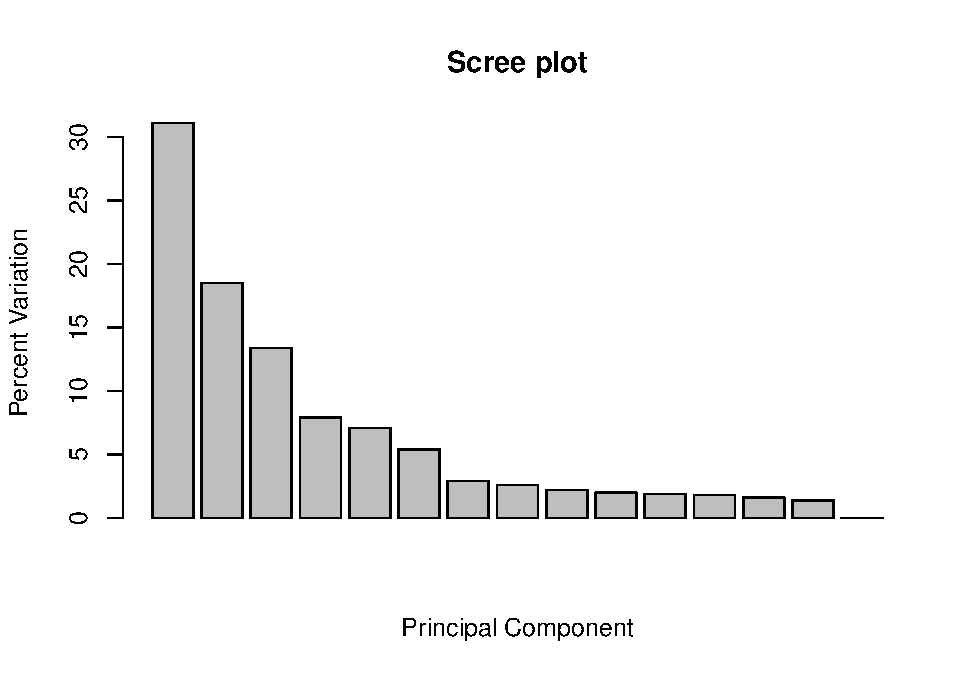
\includegraphics[height=0.25\textheight]{Layout_Report_Group4_Team4---Kopie_files/figure-latex/unnamed-chunk-11-1}
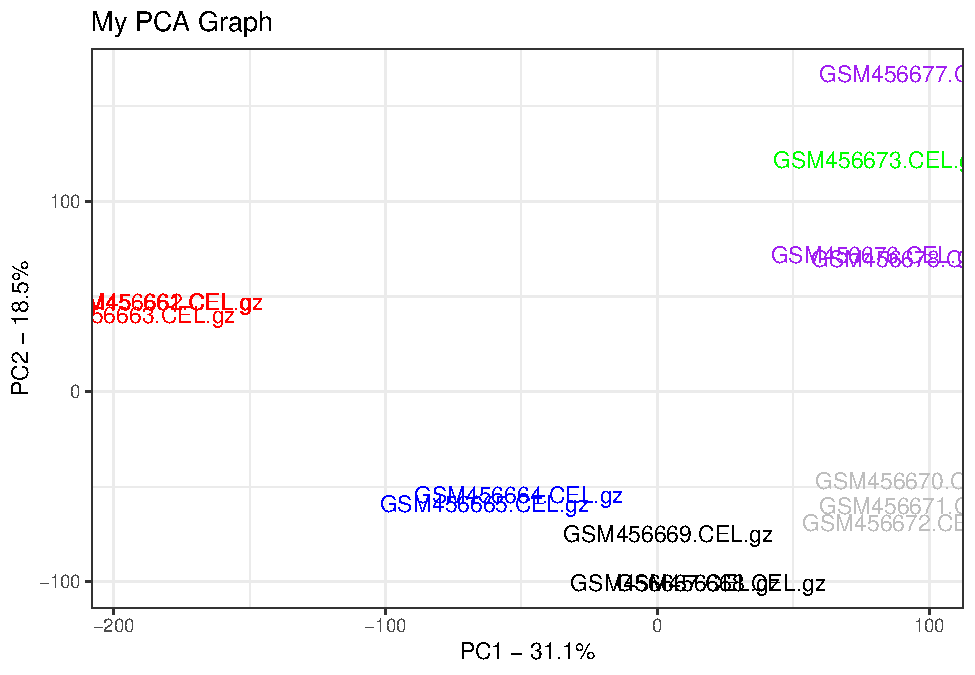
\includegraphics[height=0.25\textheight]{Layout_Report_Group4_Team4---Kopie_files/figure-latex/unnamed-chunk-11-2}

Additionally, we plotted the VSN results using boxplots. The boxplots
show us that the median of all chips align on one line, but comparing
this boxplot to the boxplot before normalization one can see that the
boxplot after VSN has more outliers.

\includegraphics[width=1\linewidth]{Layout_Report_Group4_Team4---Kopie_files/figure-latex/unnamed-chunk-12-1}

After all those steps were done, we decided to disregard 3 chips in
total (see Quality Control). We also took out the control transcripts.

\hypertarget{bovine-1}{%
\subsection{Bovine}\label{bovine-1}}

\includegraphics[height=0.25\textheight]{Layout_Report_Group4_Team4---Kopie_files/figure-latex/unnamed-chunk-14-1}

\includegraphics[width=1\linewidth]{Layout_Report_Group4_Team4---Kopie_files/figure-latex/unnamed-chunk-15-1}

\includegraphics[height=0.25\textheight]{Layout_Report_Group4_Team4---Kopie_files/figure-latex/unnamed-chunk-16-1}

\hypertarget{principal-component-analysis}{%
\section{2. Principal Component
Analysis}\label{principal-component-analysis}}

We wanted to see if the different replicates of the chips would show
high correlation if they belonged to the same stage and to see if we can
reduce the dimension of our data set. This is why we performed a
principal component analysis. Here the variables are the different genes
expressed (39281) and we have 15 samples. We transposed the matrix in
order to have the columns as the genes and the samples as the rows.
After that a scree plot was done in order to see how many principal
components are needed, which are 2 as those explain around 50\% of all
the data variance. A PCA was done using the PCA function in R. Through
the ggplot2 we can see that the first two samples (one cell stage, first
and second replicate) have excellent correlation which means one sample
and explain the entirety of the second sample. Sample 3 (GSM456663) is
also close to them. This is also the case in sample 7 and 8 (GSM456667
and GSM456668) but here the third replicate is farther than the case of
sample 3. The blastocyst first and third replicate (GSM456676 and
GSM456678) are closer to each other which hints at good correlation.
What one can notice is that the second replicate of the blastocyst
(GSM456677) is a lot farther away.

\includegraphics[height=0.25\textheight]{Layout_Report_Group4_Team4---Kopie_files/figure-latex/unnamed-chunk-18-1}
\includegraphics[height=0.25\textheight]{Layout_Report_Group4_Team4---Kopie_files/figure-latex/unnamed-chunk-18-2}

\hypertarget{hierarchical-clustering-1}{%
\section{3. Hierarchical Clustering}\label{hierarchical-clustering-1}}

Hierarchical clustering analysis is based on an algorithm that
calculates distances between the objects and forms clusters. Before we
clustered we created a distance matrix using the euclidean distance.
Based on the disance matrix we plotted a dendrogram in order to see
which cluster differ the biggest from each other. This is based on the
height of the branches. Based on the plot we can see that GSM456661 to
GSM456663 differ signficantlly from the rest of the chips. The clusters
with the biggest height difference is between GSM456661- GSM456663 and
GSM456676-GSM456678

\includegraphics[height=0.25\textheight]{Layout_Report_Group4_Team4---Kopie_files/figure-latex/unnamed-chunk-19-1}

\hypertarget{tissue-restricted-antigens-in-the-mouse-data-set}{%
\section{4. Tissue Restricted Antigens in the mouse data
set}\label{tissue-restricted-antigens-in-the-mouse-data-set}}

Through R, we were able to match our mouse data set to the TRA dataset
provided by Dinkelacker.

We plotted the frequency of the TRAs in the different tissues and found
that the highest amount of TRAs occur in testis.

\includegraphics[height=0.25\textheight]{Layout_Report_Group4_Team4---Kopie_files/figure-latex/unnamed-chunk-21-1}
Upon matching, we found that our data set contains 6188 TRAs,
transcripts and 3255 genes. After that the TRAs were matched with their
respective tissue to create a dataframe that contains the ensemble
transcripts of the TRAs, their expression value in each microarray chip
and their tissue.

\hypertarget{differential-gene-expression}{%
\section{5. Differential Gene
Expression}\label{differential-gene-expression}}

\hypertarget{mouse-1}{%
\subsection{Mouse}\label{mouse-1}}

Using limma, we performed a differential gene expression in order to see
if the deregulation of the TRAs vary in the different cell stages. The
analysis performs a t-test on the expression set and gives us the result
of the test with the p-value. The DGE simplifies this and gives us a
matrix with 3 different values that correspond to the state of the TRA.
1 is assigned if the TRA is upregulated in the contrast between the two
stages. 0 is assigned if the TRA has not significantly changed and -1 if
it is underexpressed.

Using a volcano plot, we were able to show the statistical significance
versus magnitude of fold change. The genes with a deviating fold change
can be seen on either side of the expected fold change. The genes
highlighted in red have a significant change of expression values.

\includegraphics[width=0.5\linewidth]{Layout_Report_Group4_Team4---Kopie_files/figure-latex/unnamed-chunk-24-1}
Upon plotting the deregulated TRAs of the mouse using a bar plot, we saw
that the most overexpressed TRAs are between the fourth and the eigth
cell stage. The most amount of underexpressed TRAs are between the first
and second cell stages.
\includegraphics{Layout_Report_Group4_Team4---Kopie_files/figure-latex/unnamed-chunk-25-1.pdf}
In order to visualize the tissues with most expressed TRAs we used a
treemap to categorize the large tissues and to visualize the total share
of tissues present in the fourth and eight cells stage. We saw the the
tissue with the most amount of overexpressed TRAs is the blastocyst
followed by the heart.

\includegraphics[height=0.4\textheight]{Layout_Report_Group4_Team4---Kopie_files/figure-latex/unnamed-chunk-26-1}
As our main objective is to focus on the earliest biological function,
we decided to go with the heart TRAs, as the heart is the earliest organ
that is developed. In total we have 149 TRAs in the heart, 62 of those
are overexpressed. We visualized the heart TRAs in the different cell
stages using a box-plot . Using a VENN diagram, we saw that there are
three TRAs differentially expressed that can be found in cell stage two
to four, four to eight, and eight to morula.

\includegraphics[height=0.25\textheight]{Layout_Report_Group4_Team4---Kopie_files/figure-latex/unnamed-chunk-27-1}

\hypertarget{bovine-2}{%
\subsection{Bovine}\label{bovine-2}}

\includegraphics[width=0.5\linewidth]{Layout_Report_Group4_Team4---Kopie_files/figure-latex/unnamed-chunk-29-1}

\hypertarget{gsea}{%
\section{6. GSEA}\label{gsea}}

\hypertarget{mouse-2}{%
\subsection{1. Mouse}\label{mouse-2}}

The gene set enrichment analysis was performed for the mouse data set
which was prior matched with the TRA data. The GSEA was executed with
the molecular data base MSigDB, we used the ``Hallmark gene sets' '
collection available from the website. The most overexpressed pathway,
with a 5\% p-Value, which was found with GSEA is ``Hallmark Hypoxia''.
With these results we achieved an enrichment score of 0.38 and an
associated p-Value of 4\%. This implies a scientifically enriched and
overexpressed pathway in our data set.

\hypertarget{bovine-3}{%
\section{2. Bovine}\label{bovine-3}}

The GSEA was also performed on our bovine data set without matched TRA
data. The analysis revealed two pathways which were differentially
expressed. ``Epithelial Mesenchymal Transition'' which was highly
upregulated with an ES of 0.39 and an associated p-Value of 0.1\% which
strongly suggest a significant upregulation in this gene set.
``Oxidative Phosphorylation'' is the second found pathway which is
downregulated in our data with an ES of 0.46 and a similarly associated
p-Value of 0.1\%.

\includegraphics[height=0.25\textheight]{Layout_Report_Group4_Team4---Kopie_files/figure-latex/unnamed-chunk-32-1}
\includegraphics[height=0.25\textheight]{Layout_Report_Group4_Team4---Kopie_files/figure-latex/unnamed-chunk-32-2}

\hypertarget{discussion}{%
\chapter{Discussion}\label{discussion}}

By doing a quality control on both mouse and bovine data sets, we
assessed if the microarray chips can be used to work with, or if they
all are unusable. As mentioned in the methods section, we concluded that
the mouse data set can be used if we exclude the three low quality chip,
GSM456665, GSM456674 and GSM456675. Their low quality is noticeable in
the RNA degradation plot as they cross with the other lines of the
microarrays.The only downside is, that we are only left with one
replicate of the morula cell stage, which could lead to inaccuracy. We
excluded the last bovine microarray chip as it also shows low quality.
The quality issues can be caused by dye irregularities or binding of the
of the targets to the probe. How well the bound probes to the targets
are saturated and their distance to the 3' End of the transcript can
also have an effect on the quality (Fasold and Binder, 2012) (Fasold
\emph{et. al}, 2012).

Performing a variance stabilization normalization is crucial in handling
our data, as our data set is prone to errors through the intensities.
The VSN reduces background noise and illusions (Huber \emph{et al.},
2002). Our VSN turns out to be successful, as we can see in the box
plots that the median is equal in every chip. On the other ha21nd, the
VSN produced more outliers due to the fact that the median needs to be
equal in all chips, yet the chips don't have the same expression values
in the between the different cell stages. Plotting the density
probability against the log intensity after the normalization shows to
be successful, as all the lines of the different cell stages and
replicates align, forming almost one curve. The variance stabilizaed and
normalized data can be used for further analysis.

The performed PCA shows a high correlation between the tested chips,
hence we conclude that the replicates of the chips belong to the same
cell stage. With an overall variance explanation of 50\% the PCA results
are overall satisfying. A varied gene expression of replicate sample 3
(GSM456663) would explain why this chip is not closely in the ggplot
with the other replicate of the same cell stage.This approach might also
be a possible explanation for the second replicate of the blastocyst
cell stage, which is also not near the other replicates in the plot.

We performed a clustering analysis in order to group the chips that are
most similar to each other, and to see how much the chips of different
cell stages vary. Interestingly enough we saw that the chips of the
first cell stage differ completely from the rest, as they are clustered
alone. Biologically this makes sense, as the major zygote activation did
not happen yet. In the first cell stage the cell has two gametes. The
gametes need to form a new organism that is totipotent in order to
initiate development. This happens through a process called maternal to
zygotic transition, this allows the production of zygotic gene products
instead of the maternal products (Schulz and Harrison, 2019) (Schulz
\emph{et al.}, 2019). Another thing that can be deduced from the
clustering analysis is that the GSM456677 chip (blastocyst, second
replicate) is clustered with the GSM456673 chip (morula first
replicate). A reason for this can be that through the quality control,
we excluded the second and third replicate of the morula cells due to
their low quality. This could lead to the clustering of the morula
replicate with the blastocyst replicate as the genetic material of
morula is characteristically closer to the blastocyst genetic material
than the eighth cell stage.

With the performed DGE across all stages we could see that, the highest
changes of genetic expression pattern are in the fourth and eight cell
stage. For this matter we plotted the sum of the upregulated genes
throughout the cell stages in figure (HIER BARPLOT DGE) Specifically,
the changes apply to over expressed genes in this cell stage. This
result aligned with the results by Xie \emph{et al.} which describes
that the biggest changes in genetic expression changes are to be found
after ZGA in mouse (after the second cell stage), since the maternal
transcripts are removed, and the zygotes own genetic expression derives.
We did not find any significant results in the downregulation of the
genes in the fourth and eight cell stage, the biggest downregulation of
gene transcripts ensues in the one -- two cell stage, that is why
decided to discard these results and to work henceforth with the
upregulated gene transcripts in the cell stage we focus on. Likewise, we
plotted the sum of gene transcripts with no significant change but
decided that this has no noteworthy meaning for our further analysis.

Further we performed a DGE with our mouse dataset, which was prior
matched with TRAs provided by Dinkelacker, because we hypothesized that
the biggest change of genetic expression in mouse could be in the fourth
cell stage, according to Xie \emph{et al.} The expression of TRA related
genes should also be influenced by that fact. For this matter we plotted
the sum of the upregulated genes throughout the cell stages in figure
(HIER BARPLOT VON. DGE) and the results correspond with our hypothesis,
because the most upregulated genes regarding TRA expression are in the
fourth to eight cell stage. Since the TRA expression and relevance are
yet not to be finally explained in the embryonic development and also
not in the heart development or heart depended on genes, we could not
conclude a biological relevance of this matter, apart from taking a
closer look at the tissues the TRAs are found in. We carried out a
volcano plot and could show that of the top ten underexpressed genes
transcripts which we found, four of them belong to the gene H1foo. H1foo
belongs to H1 Histone family H1foo is involved in global epigenetic
regulation and when active, will impair cell differentiation involved in
formation of condensed chromatin, which cannot be read by DNA
Polymerases H1foo is an epigenomic modulator that decondensed chromatin
and impairs pluripotency and Oocyte-specific linker histone
(ncbi.nlm.nih.gov/pmc/articles/PMC6558659/). Since a down regulated
histone activity advances the ZGA, this result aligns with the very
early ZGA of the mouse in the first and second cell stage.
(\url{https://pubmed.ncbi.nlm.nih.gov/31511251/})

Through the VENN diagram we saw that there are three transcripts that
are expressed in the cell stages two to eight. The transcripts code for
the gene Idh2, which stands for isocitrate dehydrogenase 2. The gene
codes for this enzyme which is found in the mitochondria, that catalyzes
the oxidative decarboxylation of isocitrate to 2-oxoglutarate in the
citrate cycle. In the mitochondria, it controls the mitochondrial redox
balance, which is a first line of defense against the oxidative damage.
If this balance is not held, oxidative stress can be enhanced which
results in the increase of reactive oxygen species (ROS). This can lead
to cardiac hypertrophy, which is a risk factor of heart failure (Ku
\emph{et al.}, 2015) (Jun Ku \emph{et al.}, 2015). The importance of the
Idh2 gene explains why it is expressed in the cell stages two to eight.

\hypertarget{appendix}{%
\chapter{Appendix}\label{appendix}}

\hypertarget{mouse-images}{%
\section{Mouse Images}\label{mouse-images}}

\includegraphics[height=1\textheight]{Layout_Report_Group4_Team4---Kopie_files/figure-latex/unnamed-chunk-33-1}
\includegraphics[height=1\textheight]{Layout_Report_Group4_Team4---Kopie_files/figure-latex/unnamed-chunk-33-2}
\includegraphics[height=1\textheight]{Layout_Report_Group4_Team4---Kopie_files/figure-latex/unnamed-chunk-33-3}
\includegraphics[height=1\textheight]{Layout_Report_Group4_Team4---Kopie_files/figure-latex/unnamed-chunk-33-4}
\includegraphics[height=1\textheight]{Layout_Report_Group4_Team4---Kopie_files/figure-latex/unnamed-chunk-33-5}
\includegraphics[height=1\textheight]{Layout_Report_Group4_Team4---Kopie_files/figure-latex/unnamed-chunk-33-6}
\includegraphics[height=1\textheight]{Layout_Report_Group4_Team4---Kopie_files/figure-latex/unnamed-chunk-33-7}
\includegraphics[height=1\textheight]{Layout_Report_Group4_Team4---Kopie_files/figure-latex/unnamed-chunk-33-8}
\includegraphics[height=1\textheight]{Layout_Report_Group4_Team4---Kopie_files/figure-latex/unnamed-chunk-33-9}
\includegraphics[height=1\textheight]{Layout_Report_Group4_Team4---Kopie_files/figure-latex/unnamed-chunk-33-10}
\includegraphics[height=1\textheight]{Layout_Report_Group4_Team4---Kopie_files/figure-latex/unnamed-chunk-33-11}
\includegraphics[height=1\textheight]{Layout_Report_Group4_Team4---Kopie_files/figure-latex/unnamed-chunk-33-12}
\includegraphics[height=1\textheight]{Layout_Report_Group4_Team4---Kopie_files/figure-latex/unnamed-chunk-33-13}
\includegraphics[height=1\textheight]{Layout_Report_Group4_Team4---Kopie_files/figure-latex/unnamed-chunk-33-14}
\includegraphics[height=1\textheight]{Layout_Report_Group4_Team4---Kopie_files/figure-latex/unnamed-chunk-33-15}
\includegraphics[height=1\textheight]{Layout_Report_Group4_Team4---Kopie_files/figure-latex/unnamed-chunk-33-16}
\includegraphics[height=1\textheight]{Layout_Report_Group4_Team4---Kopie_files/figure-latex/unnamed-chunk-33-17}
\includegraphics[height=1\textheight]{Layout_Report_Group4_Team4---Kopie_files/figure-latex/unnamed-chunk-33-18}

\hypertarget{bovine-images}{%
\section{Bovine Images}\label{bovine-images}}

\includegraphics[height=1\textheight]{Layout_Report_Group4_Team4---Kopie_files/figure-latex/unnamed-chunk-34-1}
\includegraphics[height=1\textheight]{Layout_Report_Group4_Team4---Kopie_files/figure-latex/unnamed-chunk-34-2}
\includegraphics[height=1\textheight]{Layout_Report_Group4_Team4---Kopie_files/figure-latex/unnamed-chunk-34-3}
\includegraphics[height=1\textheight]{Layout_Report_Group4_Team4---Kopie_files/figure-latex/unnamed-chunk-34-4}
\includegraphics[height=1\textheight]{Layout_Report_Group4_Team4---Kopie_files/figure-latex/unnamed-chunk-34-5}
\includegraphics[height=1\textheight]{Layout_Report_Group4_Team4---Kopie_files/figure-latex/unnamed-chunk-34-6}
\includegraphics[height=1\textheight]{Layout_Report_Group4_Team4---Kopie_files/figure-latex/unnamed-chunk-34-7}
\includegraphics[height=1\textheight]{Layout_Report_Group4_Team4---Kopie_files/figure-latex/unnamed-chunk-34-8}
\includegraphics[height=1\textheight]{Layout_Report_Group4_Team4---Kopie_files/figure-latex/unnamed-chunk-34-9}
\includegraphics[height=1\textheight]{Layout_Report_Group4_Team4---Kopie_files/figure-latex/unnamed-chunk-34-10}
\includegraphics[height=1\textheight]{Layout_Report_Group4_Team4---Kopie_files/figure-latex/unnamed-chunk-34-11}
\includegraphics[height=1\textheight]{Layout_Report_Group4_Team4---Kopie_files/figure-latex/unnamed-chunk-34-12}
\includegraphics[height=1\textheight]{Layout_Report_Group4_Team4---Kopie_files/figure-latex/unnamed-chunk-34-13}
\includegraphics[height=1\textheight]{Layout_Report_Group4_Team4---Kopie_files/figure-latex/unnamed-chunk-34-14}
\includegraphics[height=1\textheight]{Layout_Report_Group4_Team4---Kopie_files/figure-latex/unnamed-chunk-34-15}
\includegraphics[height=1\textheight]{Layout_Report_Group4_Team4---Kopie_files/figure-latex/unnamed-chunk-34-16}

\hypertarget{refs}{}
\begin{CSLReferences}{0}{0}
\leavevmode\vadjust pre{\hypertarget{ref-AOKI2022}{}}%
AOKI, F (2022). \href{https://doi.org/10.1262/jrd.2021-129}{Zygotic gene
activation in mice: Profile and regulation}. Journal of Reproduction and
Development 68, 79--84.

\leavevmode\vadjust pre{\hypertarget{ref-org.MM.eg.db}{}}%
Carlson, M (2022). Org.mm.eg.db: Genome wide annotation for mouse.

\leavevmode\vadjust pre{\hypertarget{ref-Ciemerych2005}{}}%
Ciemerych, MA, and Sicinski, P (2005).
\href{https://doi.org/10.1038/sj.onc.1208608}{Cell cycle in mouse
development}. Oncogene 24, 2877--2898.

\leavevmode\vadjust pre{\hypertarget{ref-dge}{}}%
Conesa, A et al. (2016). A survey of best practices for {RNA-seq} data
analysis. Genome Biol 17.

\leavevmode\vadjust pre{\hypertarget{ref-bovineux2fmousecdf}{}}%
Dai, M et al. (2005). Evolving gene/transcript definitions significantly
alter the interpretation of GeneChip data. Nucleic Acids Research
33(20), e175.

\leavevmode\vadjust pre{\hypertarget{ref-msigdbr}{}}%
Dolgalev, I (2022).
\href{https://CRAN.R-project.org/package=msigdbr}{Msigdbr: MSigDB gene
sets for multiple organisms in a tidy data format}.

\leavevmode\vadjust pre{\hypertarget{ref-Dunwoodie2009}{}}%
Dunwoodie, SL (2009).
\href{https://doi.org/10.1016/j.devcel.2009.11.008}{The role of hypoxia
in development of the mammalian embryo}. Developmental Cell 17,
755--773.

\leavevmode\vadjust pre{\hypertarget{ref-qcissues}{}}%
Fasold, M, and Binder, H (2012). Estimating {RNA-quality} using
{GeneChip} microarrays. BMC Genomics 13, 186.

\leavevmode\vadjust pre{\hypertarget{ref-affy}{}}%
Gautier, L, Cope, L, Bolstad, BM, and Irizarry, RA (2004).
\href{https://doi.org/10.1093/bioinformatics/btg405}{{affy---analysis of
Affymetrix GeneChip data at the probe level}}. Bioinformatics 20,
307--315.

\leavevmode\vadjust pre{\hypertarget{ref-vsn}{}}%
Huber, W, von Heydebreck, A, Sueltmann, H, Poustka, A, and Vingron, M
(2002). Variance stabilization applied to microarray data calibration
and to the quantification of differential expression. Bioinformatics 18
Suppl. 1, S96--S104.

\leavevmode\vadjust pre{\hypertarget{ref-Kojima_2014}{}}%
Kojima, Y, Tam, OH, and Tam, PPL (2014).
\href{https://doi.org/10.1016/j.semcdb.2014.06.010}{Timing of
developmental events in the early mouse embryo}. Seminars in Cell
Developmental Biology 34, 65--75.

\leavevmode\vadjust pre{\hypertarget{ref-Krishnan_2008}{}}%
Krishnan, J, Ahuja, P, Bodenmann, S, Knapik, D, Perriard, E, Krek, W,
and Perriard, J-C (2008).
\href{https://doi.org/10.1161/01.res.0000338613.89841.c1}{Essential role
of developmentally activated hypoxia-inducible factor a for cardiac
morphogenesis and function}. Circulation Research 103, 1139--1146.

\leavevmode\vadjust pre{\hypertarget{ref-Idh2}{}}%
Ku, HJ, Ahn, Y, Lee, JH, Park, KM, and Park, J-W (2015). {IDH2}
deficiency promotes mitochondrial dysfunction and cardiac hypertrophy in
mice. Free Radic Biol Med 80, 84--92.

\leavevmode\vadjust pre{\hypertarget{ref-Mihajlovi__2017}{}}%
Mihajlović, AI, and Bruce, AW (2017).
\href{https://doi.org/10.1098/rsob.170210}{The first cell-fate decision
of mouse preimplantation embryo development: Integrating cell position
and polarity}. Open Biology 7, 170210.

\leavevmode\vadjust pre{\hypertarget{ref-Monteleone_Cassiano_2022}{}}%
Monteleone-Cassiano, AC, Dernowsek, JA, Mascarenhas, RS, Assis, AF,
Pitol, D, Moreira, NCS, Sakamoto-Hojo, ET, Issa, JPM, Donadi, EA, and
Passos, GA (2022). \href{https://doi.org/10.1186/s12860-022-00414-9}{The
absence of the autoimmune regulator gene ({AIRE}) impairs the
three-dimensional structure of medullary thymic epithelial cell
spheroids}. {BMC} Molecular and Cell Biology 23.

\leavevmode\vadjust pre{\hypertarget{ref-BiocManager}{}}%
Morgan, M (2022).
\href{https://CRAN.R-project.org/package=BiocManager}{BiocManager:
Access the bioconductor project package repository}.

\leavevmode\vadjust pre{\hypertarget{ref-dgelimma}{}}%
Phipson, B, Lee, S, Majewski, IJ, Alexander, WS, and Smyth, GK (2016).
Robust hyperparameter estimation protects against hypervariable genes
and improves power to detect differential expression. Ann Appl Stat 10,
946--963.

\leavevmode\vadjust pre{\hypertarget{ref-R}{}}%
R Core Team (2022). \href{https://www.R-project.org/}{R: A language and
environment for statistical computing}, Vienna, Austria: R Foundation
for Statistical Computing.

\leavevmode\vadjust pre{\hypertarget{ref-RStudio:2021.9.0.351}{}}%
RStudio Team (2021). \href{http://www.rstudio.com/}{RStudio: Integrated
development environment for r}, Boston, MA: RStudio, PBC.

\leavevmode\vadjust pre{\hypertarget{ref-zygotic-transition}{}}%
Schulz, KN, and Harrison, MM (2019). Mechanisms regulating zygotic
genome activation. Nat Rev Genet 20, 221--234.

\leavevmode\vadjust pre{\hypertarget{ref-Sha_2019}{}}%
Sha, Q-Q, Zhu, Y-Z, Li, S, Jiang, Y, Chen, L, Sun, X-H, Shen, L, Ou,
X-H, and Fan, H-Y (2019).
\href{https://doi.org/10.1093/nar/gkz1111}{Characterization of zygotic
genome activation-dependent maternal {mRNA} clearance in mouse}. Nucleic
Acids Research 48, 879--894.

\leavevmode\vadjust pre{\hypertarget{ref-Takaba_2017}{}}%
Takaba, H, and Takayanagi, H (2017).
\href{https://doi.org/10.1016/j.it.2017.07.010}{The mechanisms of t cell
selection in the thymus}. Trends in Immunology 38, 805--816.

\leavevmode\vadjust pre{\hypertarget{ref-gsea}{}}%
Thomas, MA, Yang, L, Carter, BJ, and Klaper, RD (2011). Gene set
enrichment analysis of microarray data from pimephales promelas
(rafinesque), a non-mammalian model organism. BMC Genomics 12, 66.

\leavevmode\vadjust pre{\hypertarget{ref-tidyverse}{}}%
Wickham, H et al. (2019).
\href{https://doi.org/10.21105/joss.01686}{Welcome to the {tidyverse}}.
Journal of Open Source Software 4, 1686.

\leavevmode\vadjust pre{\hypertarget{ref-Xie_2010}{}}%
Xie, D, Chen, C-C, Ptaszek, LM, Xiao, S, Cao, X, Fang, F, Ng, HH, Lewin,
HA, Cowan, C, and Zhong, S (2010).
\href{https://doi.org/10.1101/gr.100594.109}{Rewirable gene regulatory
networks in the preimplantation embryonic development of three mammalian
species}. Genome Research 20, 804--815.

\end{CSLReferences}

\end{document}
